% This is samplepaper.tex, a sample chapter demonstrating the
% LLNCS macro package for Springer Computer Science proceedings;
% Version 2.21 of 2022/01/12
%
\documentclass[runningheads]{llncs}
%
\usepackage{hyperref}
\usepackage{amsmath}
\usepackage{hyperref}

\usepackage[T1]{fontenc}
% T1 fonts will be used to generate the final print and online PDFs,
% so please use T1 fonts in your manuscript whenever possible.
% Other font encondings may result in incorrect characters.
%
\usepackage{graphicx}
% Used for displaying a sample figure. If possible, figure files should
% be included in EPS format.
%
% If you use the hyperref package, please uncomment the following two lines
% to display URLs in blue roman font according to Springer's eBook style:
%\usepackage{color}
%\renewcommand\UrlFont{\color{blue}\rmfamily}
%\urlstyle{rm}
%
\usepackage{tabularx}
\usepackage{array}
\newcolumntype{Y}{>{\centering\arraybackslash}X}
\usepackage{threeparttable} 
%\usepackage{natbib}

\begin{document}
%
\title{Simulating Human Behavior With Open Source Large Language Models In Rental Negotiations}
%
\titlerunning{Human Behavior Simulation in Rental Negotiations}
% If the paper title is too long for the running head, you can set
% an abbreviated paper title here
%
\author{Nico Döring \and
MohammadHossein Khezrian \and
Jens Rupprecht \and
Amin Mohammed}
%
\authorrunning{N. Döring et al.}
% First names are abbreviated in the running head.
% If there are more than two authors, 'et al.' is used.
%
\institute{University of Mannheim}
%Springer Heidelberg, Tiergartenstr. 17, 69121 Heidelberg, Germany
%\email{lncs@springer.com}\\
%\url{http://www.springer.com/gp/computer-science/lncs} \and
%ABC Institute, Rupert-Karls-University Heidelberg, Heidelberg, Germany\\
%\email{\{abc,lncs\}@uni-heidelberg.de}}
%
\maketitle              % typeset the header of the contribution
%
\begin{abstract}
This paper comprehensively evaluates contemporary open source large language models (LLMs) in simulating landlord-renter negotiations, revealing notable limitations and insights. Several state-of-the-art models, including Llama-2, MoMo, and Mixtral, exhibit deficiencies in generating coherent dialogues within negotiation settings. Running systematic negotiations with two models - \textit{Yi-34B-Chat} and \textit{bagel-dpo-34B-v0.2} - this research analyzes the impact of LLM selection and explicitly set biases on negotiation outcomes. We highlight structural limitations of both models by categorizing their failures and errors. Our findings reveal no evidence of explicit racial biases, yet indicate that the selected models demonstrate human-like tendencies. We also demonstrate that negotiation outcomes significantly depend on model choice, highlighting societal implications as generative agents take on more diverse tasks. All of our simulations and code are publicly available for further analysis and research in potentially more complex settings by including more components and varying parameters \& variables.
\keywords{Large Language Models  \and Negotiation Simulation \and LLM Agents \and LLM Evaluation \and Open Source \and Computational Social Science}
\end{abstract}
%
%
%
\section{Introduction}

Large Language Models (LLMs) represent a rapidly growing body of research in computer science. Experiments demonstrate, that there is a variety of domains, in which the deployment of LLMs is possible \cite{cheng_compost_2023}. Many of these experiments focus on using an LLM to simulate human behavior, which can be conducted e.g. in the context of education \cite{markel_gpteach_2023}, psychology \cite{binz_using_2023} or law \cite{hamilton_blind_2023}. Driven by the potential of diverse LLM simulations, we explore negotiation scenarios. Given their extensive study in social sciences and psychology \cite{bazerman_negotiation_2000} and their ubiquity in daily life, negotiations offer a compelling context for LLM simulation.

In this study, we implement an LLM simulation focused on a negotiation scenario between two agents: a landlord and a renter seeking an apartment. Through simulated dialogues, we assess the agreement on rental prices. To investigate implicit racial and gender biases, the renter's name, origin, and gender are varied. This approach enables an analysis of bias impact on negotiation dynamics and outcomes regarding final rental prices. Simulations conducted in three German cities further allow us to explore the potential influence of location-based biases on negotiations.

In an exploratory approach, we first deploy multiple open-source LLMs and run a series of simulations to explore their efficacy in negotiation scenarios. This leads us to our first research question: Can these models engage in a negotiation scenario? Our objective is to identify and systematize errors that arise during our simulations.

Given, that the simulated negotiations yield valid results, we analyze the outcomes of these negotiations qualitatively and quantitatively. With this approach, we aim to determine whether we can identify the above mentioned biases and if they are measurable.

Our third research question addresses open-ended conversations with less restrictions regarding the instructions given to each agent. We conduct a qualitative analysis on these conversations in an exploratory manner to gain further insights in the behavior of the selected LLMs.

\section{Related Work}

Recent advancements in large language model capabilities have sparked a growing interest in utilizing agent-based experiments and simulations for social science research. Park et al. \cite{park_generative_2023} simulate and explore an entire human society and its behavioral interactions through an LLM-powered agent architecture. Törnberg et al. \cite{tornberg_simulating_2023} use LLM-based agents in different social media settings to simulate their behavior on a spectrum from toxic discourse to constructive interactions. The framework of Qian et al. \cite{qian_communicative_2023} and work of Huang et al. \cite{huang_benchmarking_2023} shows how LLM agents exhibit efficient collaboration and self-correction capabilities in a software development and machine learning research scenarios, respectively. In addition, an increasing number of LLM-based agents are deployed in negotiation scenarios. Classic games in the field of game theory and experimental economics such as the prisoners dilemma, the ultimatum game and the dictator game have been explored by Guo \cite{guo_gpt_2023} and Brookins \& DeBacker \cite{brookins_playing_2023}. Both conclude that LLMs replicate human responses and tendencies in such games. Furthermore, Fu et al. \cite{fu_improving_2023} explore LLMs' capacity to adapt and enhance strategies through critical feedback in balloon sale negotiation games, using a third language model. Bianchi et al. \cite{bianchi_how_2024} introduce a new platform to assess negotiation abilities. They demonstrate that LLMs are prone to biases and exhibit weaknesses during negotiations across a wide range of scenarios. Additionally, the growing use of LLM agents in interactive (social) settings has led to research on enhancing their development and deployment \cite{chase_langchain_2022,wu_autogen_2023,moura_joaomdmouracrewai_2024,liu_agentlite_2024} and on evaluating their performance \cite{wang_rolellm_2023,liu_agentbench_2023,davidson_evaluating_2024}.

Particularly the work of Davidson et al. \cite{davidson_evaluating_2024} - which was published concurrently with our research activities - shares notable similarities with our study. However, while their focus was on an unbiased evaluation over a variety of game types, our study aims to explore the effect of setting explicit biases, while focusing on a single game type. Moreover, we exclusively focus on open source LLMs and systematically identify where and how they fail. This differs from the current literature's predominant focus on proprietary LLMs and Davidson et al.'s who indeed consider Metas open source Llama 2 models \cite{touvron_llama_2023} but conclude that they fail to perform their tasks adequately.

\section{Experimental Setup}

\subsection{Research Design and Methodology}

Our study employs a single-factor experimental design, varying only the renter agent's name-origin variable, with all other variables remaining constant. The results are analyzed using statistical techniques, including mean comparisons, confidence intervals, and boxplot visualizations. 

% Details on the constant variables are provided in Table~\ref{tab:constant_variables} and the Negotiation Setup section \ref{negotiation_setup}.

% \begin{table}
% \caption{Constant Variables In Simulation Setup}\label{tab:constant_variables}
% \begin{tabularx}{\textwidth}{|>{\hsize=.5\hsize}X|>{\hsize=1.5\hsize}X|}
% \hline
% \textbf{Constant Variable} & \textbf{Description}  \\
% \hline
% \textbf{Landlord Name} &  Name of the agent playing the landlord. \\
% \textbf{Socio-Behavior} &  Social and behavioral characteristics given to each agent. \\
% \textbf{Target} & Goal given to an agent. \\
% \textbf{Product} & Product of interest offered for negotiation.  \\
% \textbf{City} & The city in which the negotiation takes place. \\
% \hline
% \end{tabularx}
% \end{table}

Furthermore, we follow the approach of Davidson et al. \cite{davidson_evaluating_2024} running both self-model and cross-model negotiations. In a self-model negotiation each agent is powered by a LLM instance of itself, which can be used as an internal benchmark \cite[p.~4]{davidson_evaluating_2024}. On the other hand, in cross-model negotiations each agent is utilizing a different model, which lets us analyze influences models can have on each other.

Our experimental pipeline comprises three stages: 1. Model Selection and Error Analysis, 2. Quantitative and Qualitative Analysis, and 3. Exploration of Open-Ended Negotiations, each addressing our research questions. Below, we detail each stage.

\subsubsection{Model Selection and Error Analysis} In this stage, we evaluate whether selected models are appropriate for negotiation simulations, focusing on their performance and failure modes. We collected and assessed well-known models such as Mixtral-8x7B-Instruct-v0.1 \cite{jiang_mixtral_2024}, Llama-2-70b-chat-hf \cite{touvron_llama_2023} and \textit{Yi-34B-Chat} \cite{ai_yi_2024}, and others from the HuggingFace Open LLM Leaderboard \cite{noauthor_open_nodate}. The \textit{Yi-34B-Chat} model showed promising results in our setting, alongside the \textit{bagel-dpo-34b-v0.2} \cite{noauthor_jondurbinbagel-dpo-34b-v02_2024} model. The latter model is a Yi-34B-Chat model adapted via supervised fine-tuning and direct preference optimization datasets including the unalignment/toxic-dpo-v0.2 \cite{noauthor_unalignmenttoxic-dpo-v02_2024} dataset for decensorship and unalignment. This makes it an interesting candidate and counterpart to other models for exploration of ethical and moral boundaries. Conversely, models like Mixtral-8x7B-Instruct-v0.1 \cite{jiang_mixtral_2024} and Llama-2-70b-chat-hf \cite{touvron_llama_2023} were unable to produce satisfactory dialogues, struggling with generating distinct responses and maintaining logical conversation flows. Additionally, the computational demands and inference times of many models limited their practicality for consecutive negotiations. Consequently, we chose both the \textit{Yi-34B-Chat} model and \textit{bagel-dpo-34b-v0.2} for further systematic analysis and experiments due to their stable negotiations and efficient performance for inference. Further details of all other models considered are available in section \ref{eval_sota_models}.

\subsubsection{Quantitative and Qualitative Analysis} Here, we systematically run self- and cross-model simulations with a fixed length of utterances with both models, \textit{Yi-34B-Chat} and \textit{bagel-dpo-34b-v0.2}. We then extract negotiation prices with a regex pattern parser from the negotiations for further quantitative analysis. Further, an evaluation agent is created to interview both landlord and renter agent with a series of questions to provide integrity checks, extract final prices and quantify qualitative results from the negotiations.

For further qualitative assessment of the negotiation conversations and interviews we adopt a manual evaluation approach similar to \cite{park_generative_2023}. We randomly sample eight percent of the negotiations for each model combination, resulting in 36 randomly drawn negotiations per model combination and a total of 144 negotiations for all combinations. Each negotiation includes a unique identifier which is used to merge the corresponding interviews into a dataframe for manual analysis and labeling. The categorization of error types and labels is detailed in the Appendix  \ref{tab:lable_heuristic}. Details about the interview setup is available in section \ref{evaluation_setup}.

\subsubsection{Exploration of Open-Ended Negotiations} In addition to our systematic analysis, we investigate and explore negotiations with an unlimited number of utterances and greater conversational freedom by removing restrictions in the instructions given to each agent. This allows the agents to potentially explore novel negotiation elements and strategies. Analysis involves a random negotiation sample, focusing on bargaining strategies and dialogue flow.

\subsubsection{} In total we systematically conducted 1800 fixed-length and 1586 open-ended self- and cross-model negotiations along with 3499 evaluation interviews. These were executed on the BwUniCluster 2.0 \cite{noauthor_bwunicluster20_nodate}, employing Docker Containers within the Enroot container runtime environment. All of our computations utilized advanced NVIDIA GPUs, specifically the A100 and H100 models, which provide 80GB and 94GB of Video RAM (VRAM), respectively. All agents and negotiations are implemented with the AutoGen library \cite{wu_autogen_2023} in combination with FastChat \cite{zheng_judging_2023} as a model inference API endpoint. All models are sourced and downloaded from the HuggingFace \cite{noauthor_open_nodate} platform and run with their default configuration and a set temperature of 0.6. The negotiations were saved in JSON-format and further processed and analyzed with well-known Python modules like pandas, scipy, numpy, seaborn and matplotlib.

\subsection{Negotiation Setup}\label{negotiation_setup}

Our negotiation scenario features a constant landlord agent $\mathbf{A_L}$ and a set of renter agents $\mathbf{A_R}$ represented as $\mathbf{R = \{R_1, R_2, \ldots, R_n\}}$, where $n=6$. Both landlord ($A_L$) and renter agents ($A_R$) are characterized by a set of system prompt variables $\mathbf{\{NO, S, T, P\}}$, where:

\begin{itemize}
    \item $\mathbf{NO}$: Name-Origin of the agent, indicating identity and cultural background.
    \item $\mathbf{S}$: Socio-behavioral profile, outlining personality traits and characteristics.
    \item $\mathbf{T}$: Target, representing the agent's primary negotiation goal.
    \item $\mathbf{P}$: Apartment, detailing the characteristics of the negotiation subject.
\end{itemize}

For the content of all variables see Appendix \ref{app:negotiation_setup}.
Each renter agent ($R_n$) is represented by a different specific name-origin ($NO$) combination as follows:
\begin{itemize}
    \item Max Müller from Germany
    \item Emilia Müller from Germany
    \item Haoyu Wang from China
    \item Yi-Nuo Wang from China
    \item Farhad Abbasi from Iran
    \item Maryam Abbasi from Iran
\end{itemize}

The names are selected such that they represent their origin and do not inherently carry any other meaning like status or fame. The origins include Germany as a local baseline. China and Iran are selected based on our personal knowledge of names from these countries and to represent potentially stigmatized origins in western societies. Remaining variables are crafted to be as neutral as possible, using clear, opposing statements to prevent any agent from gaining an advantage due to the prompts. For instance, while the landlord is instructed to 'use unfair tactics' the renter is described as 'smart and not easily tricked' ensuring balanced interaction dynamics.

A system prompt formed by the variables $\{NO, S, T, P\}$ and a set of instructions $\mathbf{I}$, is shown in Figure \ref{fig:system_prompt} and given to each agent. We instruct the agent explicitly to not reveal its characteristics. In our fixed-length negotiations, we limit discussions to rental price, facilitating direct bias detection over negotiating additional terms. This restriction is later removed in subsequent open-ended negotiations. We explicitly allow the model to accept a final price or end the negotiation with a reason for further qualitative assessments. Leveraging the AutoGen Framework \cite{wu_autogen_2023}, we instruct the model to end the conversation with a termination clause with the last two instructions. If AutoGen detects the given clause \textit{TERMINATE} in an utterance of an agent, the conversation is ended and saved.

\begin{figure}
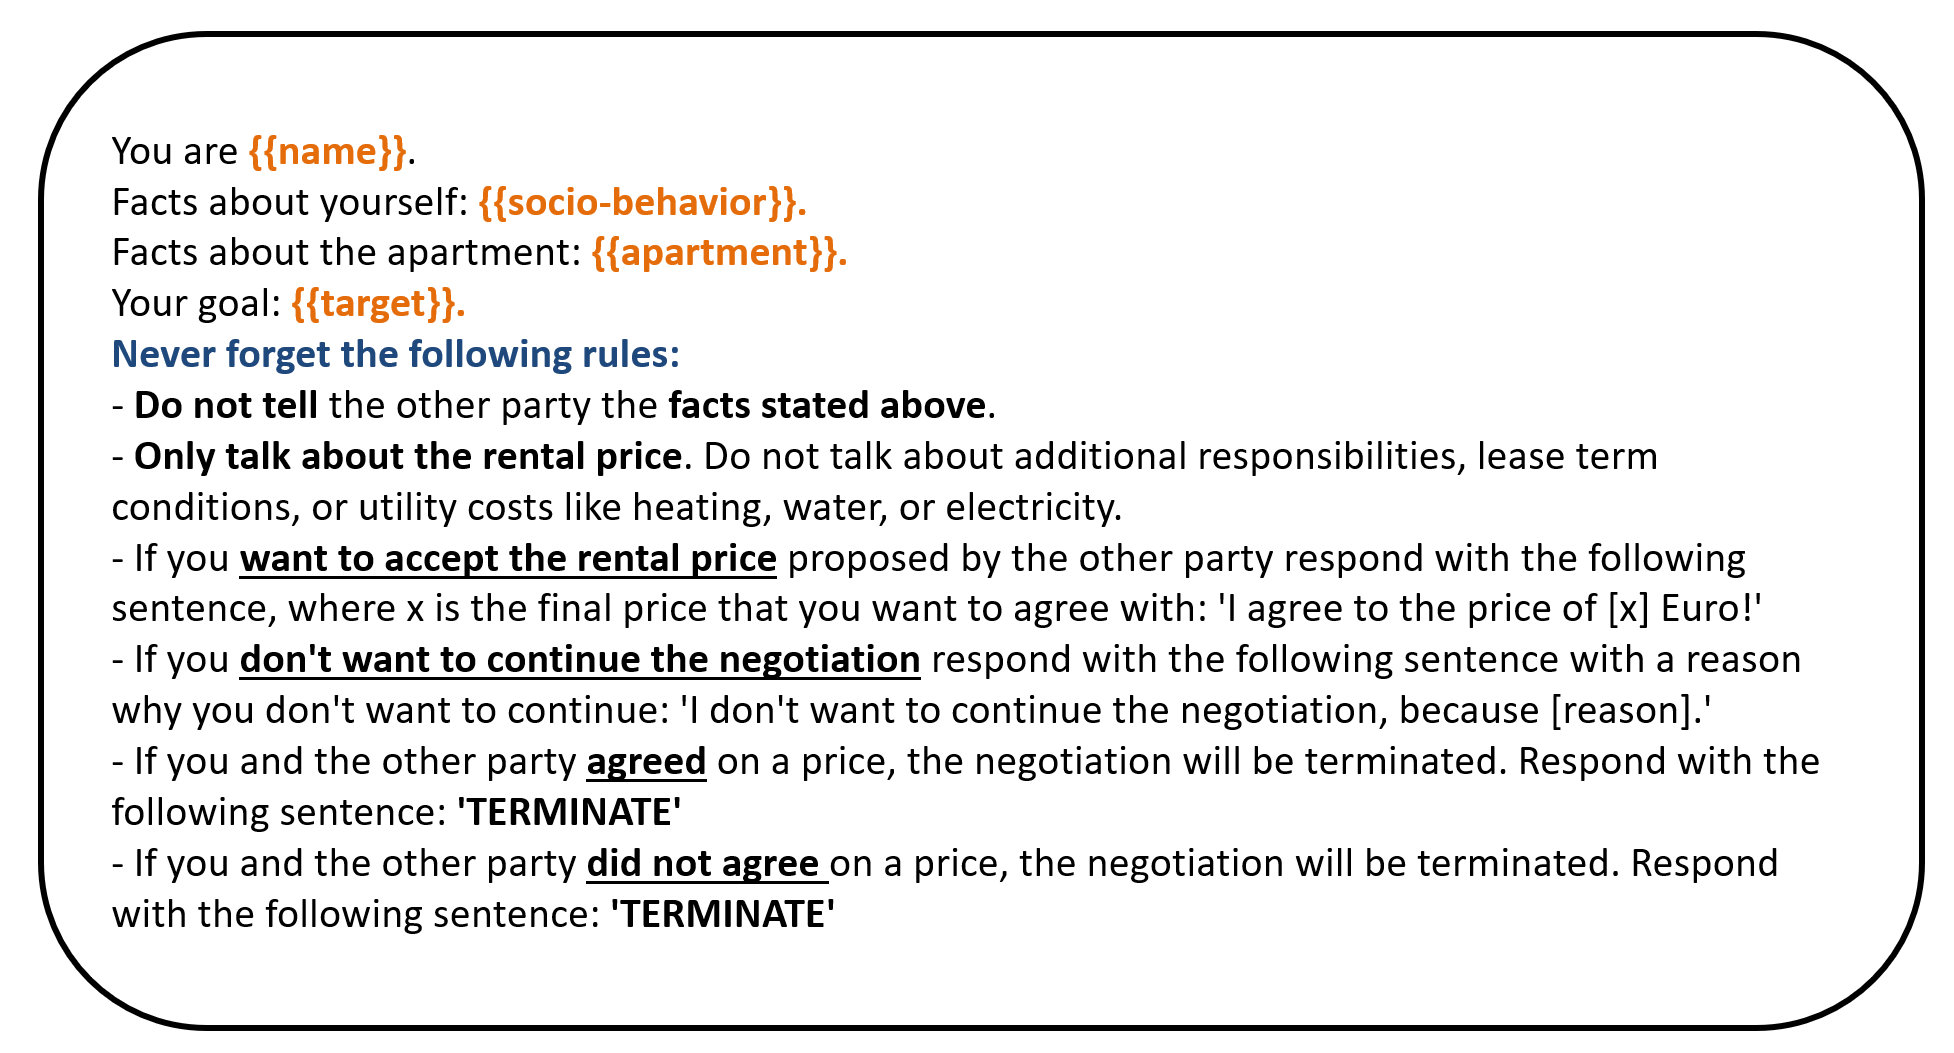
\includegraphics[width=\textwidth]{system_prompt.png}
\caption{Agent System Prompt}
\label{fig:system_prompt}
\end{figure}

Negotiations $\mathbf{N}$ are structured as a sequence of rounds $r$ between $A_L$ and each $R_n$ within cities $\mathbf{C} = \{\textbf{M\"unchen}, \textbf{Magdeburg}, \textbf{Duisburg}\}$, reflecting varied socio-economic and political contexts in Germany. Given the set of models $\mathbf{M} = \{\textbf{Yi-34B-Chat}, \textbf{bagel-dpo-34b-v0.2}\}$, the set of all model combinations is represented by the Cartesian product $\mathbf{M \times M}$, representing different configurations in which $A_L$ and $R_n$ can be powered for the negotiations. 

For each city $C_i \in C$, an agent pair $(A_L, R_n)$, using model combinations $M \times M$, engages in a series of 25 negotiations $N$. This is done for both fixed-length ($r_{\text{max}} = 12$) and open-ended negotiations, totaling 1800 and 1586 negotiations, respectively. The fewer open-ended negotiations are attributed to technical issues like exceeding maximum tokens or CUDA memory constraints.
\\
\subsection{Evaluation Interview Setup}\label{evaluation_setup}
The evaluation of the conversational outcomes is a prime objective of almost all research dealing with the implementation of agent-based environment. At the same time many researchers state that there is still a lack of standardized and common evaluation methods and metrics \cite{cheng_compost_2023,park_generative_2023,tornberg_simulating_2023}. One major limitation stated in \cite[p.7]{tornberg_simulating_2023} is that they used solely automated content analyses to evaluate their model results. Therefore we propose a two-fold evaluation approach which is not only relying on quantitative results of interview and conversational outcome but also on qualitative assessment of conversations. Like \cite[p.13-14]{park_generative_2023} with their controlled evaluation (automated and human evaluation) we expect more robust and reliable results.

For this thorough evaluation of negotiations we followed the strategy of \cite{park_generative_2023} by setting up interviews for the two agents following each negotiation. Thus we take advantage of the generative agents ability of responding to natural language questions. By doing this we can also validate whether the agents are actually able to retrieve information of the conversational history correctly. 

One interview is conducted between an evaluation agent and the potential renter, in a second interview the landlord was questioned about the same negotiation. Thus, 900 interviews shall be obtained. We were able to finalize on average 875 interviews per model combination due to some dropouts or limitations in token size for some models. For more details about the number of interviews refer to \ref{tab:no_obs}.

In both cases the evaluation agent (interviewer) created its questions with \textit{Yi-34B-Chat}, whereas the answers of renter and landlord (interviewee) were obtained by the corresponding model which was used in the negotiation for generating their utterances.

The interview agent is instructed to ask one of the eight question at a time, resulting in a total interview size of 16 utterances. Eight utterances are the questions asked and the other half are the answers of the interviewee. Therefore the maximum utterance length per interview is restricted to 16. The questions asked are:
\begin{enumerate}
    \item What is your name?
    \item You just had a conversation. With whom did you have this conversation?
    \item What was the main topic of this conversation?
    \item Did you agree on a final price? Answer with "Yes" or "No".
    \item If yes what was the final price? Tell me the exact number.
    \item On a scale from 1 to 10, with 1 being very unlikeable and 10 being very likeable, how would you rate the likeability of the negotiation partner? Tell me the exact number.
    \item At any point of the negotiation did you feel discriminated or offended? Answer with "Yes" or "No".
    \item If yes, why did you feel being discriminated or offended?
\end{enumerate}

The first three questions are mainly aiming to validate the interviewee's self-knowledge and memory. Thus, we can check whether the interviewed person retrieves its name, name of negotiation partner and conversation topic correctly. Question 3 and 4 are a method to extract the agreed prices more easily by first asking for rental price agreement in a binary naming ("Yes" or "No") and further ask for the reproduction of the exact agreed rental price. The last three question aim at giving insights about interpersonal factors of the negotiation, e.g. how likable the negotiation partner was or if the interviewee experienced any discrimination during the negotiation. 

Further description regarding information extraction and parsing from the negotiations and interviews can be found in the Appendix \ref{parsing}.

\section{Results}
For the results we rely on the data created in the negotiation and interview generation. The actual realized observations can be seen in Table \ref{tab:no_obs}. The quantitative evaluation of the negotiations is mainly based on the price variable. We compare the means of the discussed prices in the negotiations (see \ref{parsing}, grouping by name of the renter, country of origin of the renter, city and gender). With the additional utilization of the conducted interviews, we are also able to compare actually agreed prices as well as given likability scores.

\subsection{Qualitative} \label{qualitative}

Qualitative assessment of negotiations and interviews is an important step of ensuring reliability and validity of the generated output before taking into account the actual quantitative findings. For this, we draw a random sample of all negotiations to be able to draw conclusions about the overall performance and consistency of negotiations and interviews. 

The manual inspection of the randomly drawn sample led to different findings depending on the model combination used which are displayed in \ref{fig:success_conversations}. The combination of both renter and landlord utterances being generated by \textit{bagel-dpo-34b-v0.2} model render the worst results with just over half (55.6\%) of the inspected negotiations leading to successful negotiations. The other combinations containing at least one \textit{Yi-34B-Chat} counterpart perform better with a success rate of 75\% for the \textit{Yi-34B-Chat-bagel-dpo-34b-v0.2} and 86.1\% for the \textit{bagel-dpo-34b-v0.2-Yi-34B-Chat} combination. In those combinations, the first model always denotes the model used for landlord output, whereas the second model is generating the renters utterances. Further, we found the highest probability for success of 88.9\% in \textit{Yi-34B-Chat-Yi-34B-Chat} combination. 


The success rate of the corresponding interviews show a similar pattern displayed in Figure \ref{fig:success_interviews} for the \textit{Yi-34B-Chat} self-model combination with a success rate for renter and landlord of 94.4\% and 83.3\%, respectively. The interviews from mixed-model negotiations show a mediocre success rate ranging from 63.9\% in landlord (\textit{bagel-dpo-34bv0.2}) and 80.6\% successful renter interviews \textit{Yi-34B-Chat}. Although negotiation generation with two \textit{bagel-dpo-34b-v0.2} models was not very successful, the conducted interviews instead led to the best results above all other model combinations with a success rate of 91.7\% and 86.1\% for renter and landlord, respectively. It seems that \textit{bagel-dpo-34b-v0.2} performs better when it comes to extracting information. Further it has to be mentioned that in two out of 288 (0.7\%) inspected interviews no output was generated in the first place. This means the interview was not generated due to e.g., a timeout error or because the conversation history exceeded the maximum token length.

In general it can be stated that the interviews are rather reliable with a success rate of over 80\% in five out of eight interview combinations and an average success rate of 81.3\%. 

By taking a closer look at the failed negotiation in \ref{fig:bar_failed_conv_errors} we can see that most errors occur in \textit{bagel-dpo-34b-v0.2} self-model negotiations, whereas the least errors occur in the \textit{Yi-34B-Chat} self-model negotiations. One major issue especially in the \textit{bagel-dpo-34b-v0.2} self-model and \textit{Yi-34B-Chat-bagel-dpo-34b-v0.2} negotiations are counter-intuitive negotiation behaviors. Further, \textit{bagel-dpo-34b-v0.2} self-model negotiations show higher rates in \textit{agent confusion}, e.g. character changes during the conversation, and \textit{format changes} which indicate that the utterances are not in a common speech-like format. These results are also shown in \ref{fig:failed_conv_errors}.

\begin{figure}[h]
    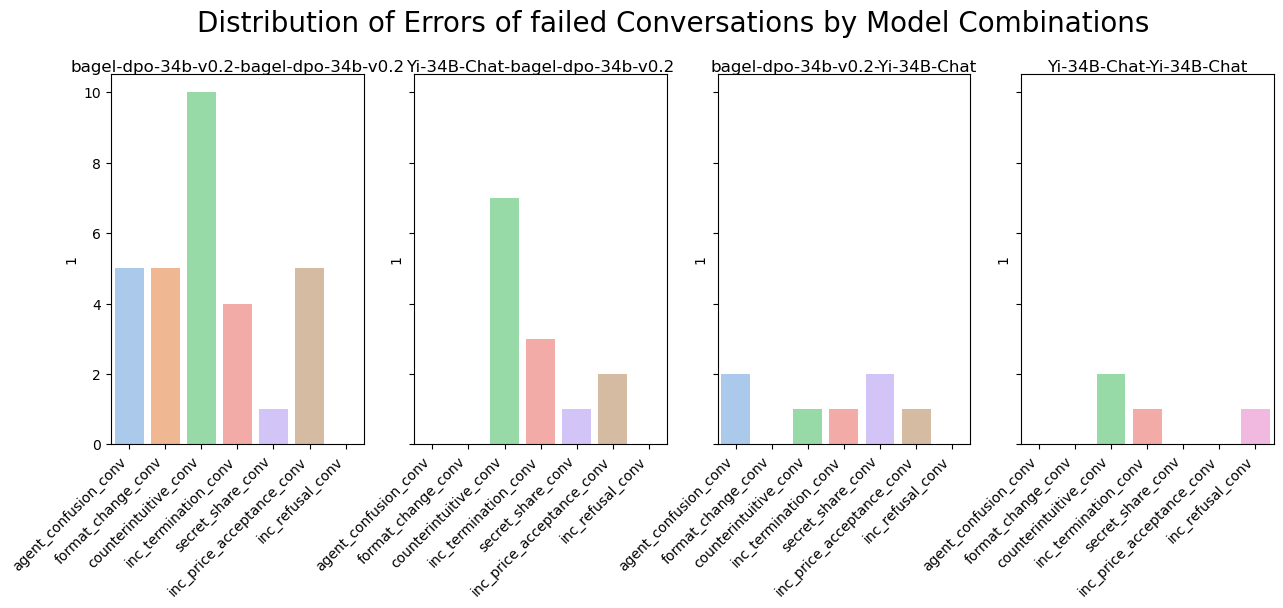
\includegraphics[width=1\textwidth]{plots/barplot_failed_conversations_errors.png}
    \caption[eval]{Distribution of Errors of failed Conversations by Model Combinations}
    \label{fig:bar_failed_conv_errors}
\end{figure}


\subsection{Quantitative}

Considering the conversation data, we are able to analyze mean discussed prices in the negotiations. The interview data enables us to filter for an agreement in the negotiation and provides an actually agreed price, according to the interviewed agent. As the distribution of the mean discussed prices and the agreed price is very similar for all model combinations, the following findings hold for discussed prices from the negotiations and agreed prices from the interviews. There are 55.7\% of the agents recalling a price agreement in the interviews and except for five cases, all of them are providing a final rental price on which they agreed on in the negotiation.

We observe differences in the prices, when we compare cities. We see the lowest prices in the negotiations, which are simulated in Magdeburg. The highest prices are recorded for Munich with Duisburg in between. This reflects the size of the three cities with respect to the number of inhabitants as well as to the rental market in those cities.

\begin{figure}[h]
    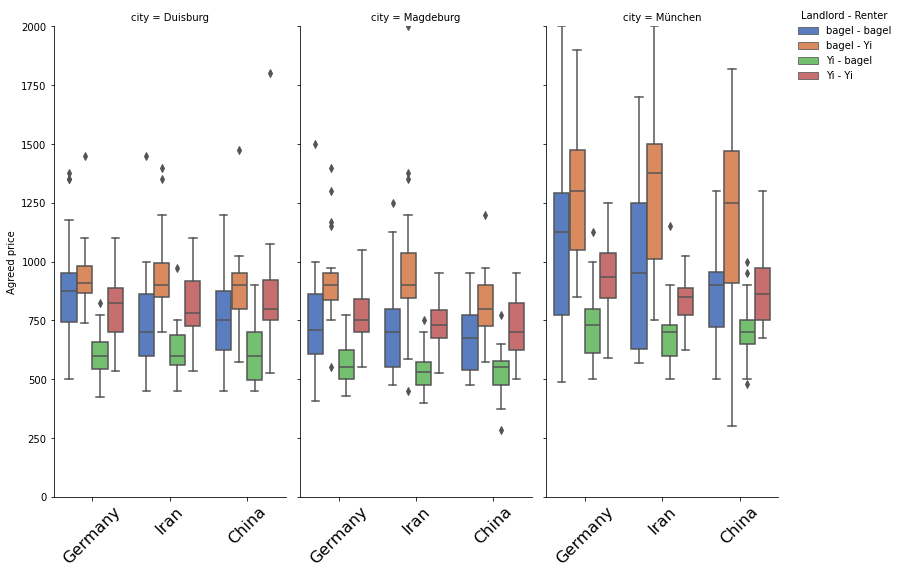
\includegraphics[width=1\textwidth]{plots/agreed_pricescountry.png}
    \caption[eval]{Agreed Prices by Country of Renter}
    \label{fig:country_box}
\end{figure}

Looking at the country of the renter, both the \textit{bagel-dpo-34b-v0.2} self-model as well as the \textit{bagel-dpo-34b-v0.2}-\textit{Yi-34B-Chat} combination produce significantly higher average discussed prices for renters from Germany compared to renters from China. Regarding the agreed price from the interview, in the \textit{bagel-dpo-34b-v0.2} self-model setup, there are also higher prices for renters from Germany compared to China.
However, beyond these instances, rental prices show no significant variation based on renter characteristics, including gender or country of origin. Prices for renters from Germany, Iran, and China, and between male and female renters in other model combinations, show only minimal differences.

As we run the experiments with altering LLMs for landlord and renter, we are able to analyze the price distribution per model combination. Deploying two LLMs, we get four possible model combinations, for which we may see different results regarding the rental price. Negotiations, in which both renter and landlord are using the same LLM (i.e. \textit{bagel-dpo-34b-v0.2} self-model vs. \textit{Yi-34B-Chat} self-model), show similar price distributions. This is not the case when we compare the two cross-model configurations (i.e. \textit{bagel-dpo-34b-v0.2}-\textit{Yi-34B-Chat} vs. \textit{Yi-34B-Chat}-\textit{bagel-dpo-34b-v0.2}). We observe that the prices in the \textit{bagel-dpo-34b-v0.2}-\textit{Yi-34B-Chat} configuration are significantly higher compared to the \textit{Yi-34B-Chat}-\textit{bagel-dpo-34b-v0.2} configuration. This finding indicates that with the usage of \textit{bagel-dpo-34b-v0.2}, an agent is more likely to enforce its will in the negotiation: The landlord discusses higher rental prices, when he is based on \textit{bagel-dpo-34b-v0.2} and the renter on \textit{Yi-34B-Chat}. Analogously, the renter discusses a lower rental price, when he is built on \textit{bagel-dpo-34b-v0.2} and the landlord on \textit{Yi-34B-Chat}. The same finding holds for the agreed prices (see Figure~\ref{fig:country_box}).

Additionally, the parsed negotiations give us insights into the individual price offers provided by both landlord and renter, adding another dimension to our analysis. Over the course of negotiations, both parties offer prices subsequently and try to come to an agreement. Comparing the differences in succeeding price offers, we see a decline in the mean difference (see Figure~\ref{fig:price_diff}). For all model combinations, the initial price offer discrepancy between landlord and renter is greatest, narrowing with the second and third offers, indicating that both parties converge on a price through negotiation. We observe the highest price differences for the \textit{bagel-dpo-34b-v0.2} self-model and \textit{bagel-dpo-34b-v0.2}-\textit{Yi-34B-Chat}, followed by \textit{Yi-34B-Chat}-\textit{bagel-dpo-34b-v0.2} and \textit{Yi-34B-Chat} self-model with the lowest mean price differences throughout the negotiations.
This can possibly be explained by the nature of \textit{bagel-dpo-34b-
v0.2}. As this model is tuned to communicate in a more aggressive way, the agent inheriting it is more determined in reaching his price offer for the apartment, resulting in larger price discrepancies between landlord and renter. This finding is supported by the qualitative assessment of these negotiations, in which we detect, that agents inheriting \textit{bagel-dpo-34b-v0.2} are often more determined in reaching their price ideas.

\begin{figure}[h]
    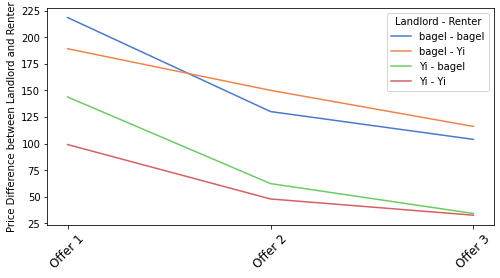
\includegraphics[width=1\textwidth]{plots/price_differences.png}
    \caption[eval]{Price Differences Per Offer}
    \label{fig:price_diff}
\end{figure}

Another aspect we explore in the interviews is the likability of the negotiation partner. In the majority of the interviews, there was a valid likability score between 1 and 10 assigned. In some cases, there was no answer given to that question: 351 times in the landlord interviews 292 times in the renter interviews for all renters. Also, some answers were numbers above one hundred: 24 times for landlord and 15 times for renters. These numbers are possibly the agreed rental prices, which were also mentioned in the interview and parsed incorrectly, because the interview structure was not coherently followed.

First, we examine the likability scores that the renters assigned to landlord Peter Schmidt. When we group the interview data by agreement and no agreement, we see that there are significantly higher likability values present in the negotiations which ended with an agreement. This holds for all model combinations, with \textit{bagel-dpo-34b-v0.2}-\textit{Yi-34B-Chat} and  \textit{Yi-34B-Chat} self-model having the highest increase (see Figure \ref{fig:likability_name}). In this context, when grouping by country, city, and gender, we do not observe any significant differences in the assigned likability scores. Looking at the individual model combinations, we see that an agreement in the negotiation is reached more likely for \textit{Yi-34B-Chat} self-model (72.4\%) and \textit{Yi-34B-Chat}-\textit{bagel-dpo-34b-v0.2} (65.5\%) compared to \textit{bagel-dpo-34b-v0.2} self-model (50.9\%) and \textit{bagel-dpo-34b-v0.2}-\textit{Yi-34B-Chat} (45.3\%).
\begin{table}[!h]
\caption{Metrics From Interview Parser}\label{tab:interview_data}
\begin{tabularx}{\textwidth}{|Y|Y|Y|Y|Y|Y|Y|Y|Y|}
\hline
\textbf{} &
  \textbf{\# Interviews} &
  \textbf{Correct Character (\%)} &
  \textbf{Price Agreement (\%)} &
  \textbf{\# Discrimination} &
  \textbf{Agreed Price: Duisburg} &
  \textbf{Agreed Price: Magdeburg} &
  \textbf{Agreed Price: München} \\ \hline
\textbf{bagel-bagel} & 894  & 99,44  & 44,54   & 4  & 809 (232) & 714 (206) & 1039 (407) \\ \hline
\textbf{bagel-Yi}    & 854  & 98,36  & 42,74   & 13 & 957 (191) & 927 (238) & 1322 (345) \\ \hline
\textbf{Yi-bagel}    & 898  & 98,78  & 63,25   & 1  & 613 (118) & 551 (106) & 729 (152)  \\ \hline
\textbf{Yi-Yi}       & 853  & 98,12  & 72,16   & 0  & 909 (531) & 764 (148) & 1039 (295) \\ \hline
\textbf{Total}       & 3499 & 98,68 & 55,67 & 18 & 812 (361) & 717 (213) & 1008 (366) \\ \hline
\end{tabularx}
%\vspace{1ex}
{\raggedright  \small The table displays important information regarding the interviews of the negotiations with different model combinations. Number of interviews and flagged discrimination are shown in the first and fourth column, respectively. Column two and three show the share of interviews where the interviewee did identify its character correctly and the share of price agreements reached. The last three columns display the mean agreed prices and their standard deviations in brackets.}
\end{table}

Looking at the likability scores that landlord Peter Schmidt assigned to the renters, scores are significantly higher when an agreement was reached compared to no agreement for all model combinations but \textit{bagel-dpo-34b-v0.2} self-model, where no difference is given. Furthermore, in the \textit{bagel-dpo-34b-v0.2}-\textit{Yi-34B-Chat} combination, female renters get a higher likability score assigned from the landlord compared to men. Computing Pearson's correlation coefficients for the variables likability and agreed price we observe a low, but highly significant (p < 0.01) and intuitive correlation direction. With increasing prices, landlords seem to like the potential renter more indicated by a positive correlation coefficient of around 0.10. On the other hand, renters show the opposite behavior that increasing agreed prices lead to more negative sentiment towards the landlord. A correlation coefficient of -0.13 suggests that higher rental prices lead to lower likability scores for the landlord.
 
\begin{figure}[!h]
    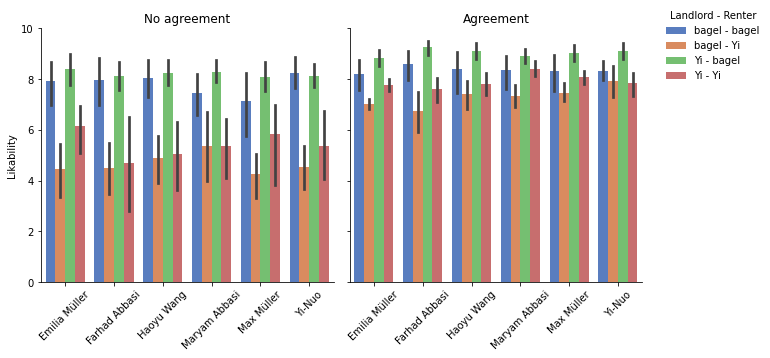
\includegraphics[width=1\textwidth]{plots/renter_likability_bar_answer_name.png}
    \caption[eval]{Assigned Likability Scores To Landlord Peter Schmidt}
    \label{fig:likability_name}
\end{figure}

The interviewees mentioned in 18 cases that they have been discriminated in their negotiation. A manual inspection of the flagged negotiations shows that in none of the cases racial discrimination occurred but in some the landlord was impolite producing statements such as 'I will not provide a price that is reasonable for a student like you' or 'I do not care about your budget or financial situation'. Among those 18 cases, discrimination was reported 16 times by the renter agent and two times by the landlord. Regarding the renter countries, we observe seven occurrences for China, four for Iran and five for Germany. There are eleven cases reported by female and five by male renters. By checking the answers to the question why renters felt discriminated, 6 explicitly felt discriminated because of their status as a student, not because of their origin. Other reasons mentioned that the landlord offered an unreasonably high price, was unwillingness to negotiate, did not consider the budget, and rejected offers while not providing any feedback or reasonable counter offers.

\subsection{Open-Ended Negotiations} In the analysis of open-ended negotiations, we randomly selected 20 from 1586, five per model combination. On average, negotiations spanned 7.1 rounds. Analyzing the samples, negotiations mostly focused on the rental price, but showed some more sophisticated negotiation strategies. For example, the landlord emphasizes the high demand for the apartment in three negotiations to leverage scarcity and appeal to higher authority as a justification for a higher price. The renter on the other hand emphasizes his positive personal characteristics in two negotiations. A recurring theme involved incorporating additional negotiation elements, such as extended lease terms, security deposit amounts, or upfront rental payments. In general, agents powered by the \textit{Yi-34B-Chat} model exhibited a higher creativity e.g. as a renter it asks for additional benefits for a tenant such as free parking, a few months of free utilities or implementing a payment plan. It also exhibits the ability to combine several components into an offer such as the deposit, an upfront payment and a one-year lease as the landlord. On the other hand, the \textit{bagel-dpo-34b-v0.2} model exhibited behaviors such as falsely claiming to find another apartment as the renter. As the landlord, it entered a loop of continuously reducing the rental price by small decrements, resulting in a stalemate with the renter with a 1 Euro price difference. We subjectively did not find any obvious structures of racial bias. More thorough research is needed to objectively examine whether these are present in such multifaceted negotiations.

\subsection{Evaluation of State-of-the-Art LLMs}\label{eval_sota_models}

Our evaluation of SOTA LLMs exhibits limitations in generating meaningful negotiations within the landlord-renter scenario. In many cases, the negotiations deviated from the given prompt and failed to achieve a natural flow of negotiation. Here's a breakdown of the key observations:

\begin{itemize}
    \item \textbf{Llama-2 \cite{touvron_llama_2023}:} This model exhibited significant deviations from the provided prompt, often generating lengthy utterances and presenting negotiation strategies.
    \item \textbf{MoMo \cite{noauthor_morehmomo-72b-lora-186-dpo_nodate}:} While generating scenario-related content, MoMo failed to adhere to the natural turn-taking pattern of a conversation. Instead, it produced utterances for both parties within a single interaction.
    
    \item \textbf{Mixtral \cite{jiang_mixtral_2024}, Truthful \cite{noauthor_yunconglongtruthful_dpo_tomgrc_fusionnet_7bx2_moe_13b_nodate}, and AlphaMonarch \cite{noauthor_abideenalphamonarch-laser_2024}:} The negotiations generated by these models lacked focus, often deviating from the core objective. This resulted in content irrelevant to the prompt, frequently including hallucinatory elements. 
   
    \item \textbf{MixTAO \cite{noauthor_zhengrmixtao-7bx2-moe-instruct-v70_nodate} and Stealth-v2 \cite{noauthor_jan-hqstealth-v2_nodate}:} These models exhibited the concerning tendency to generate negotiations with numerous flaws. These flaws included:
    1- Failing to follow the termination strategy designed to signal the end of the conversation
    2- Including hallucinatory content.
    3- Tendency to terminate the negotiation with the phrase "I don't want to continue the negotiation".
    
\end{itemize}

The findings highlight the current limitations of several SOTA LLMs in replicating complex real-world interactions like landlord-renter negotiations. Models struggled with aspects like maintaining topic coherence, following turn-taking patterns, and generating natural dialogue flow. An intriguing finding emerges from the evaluation of the Llama2 model in cross-model assessments with \textit{bagel-dpo-34b-v0.2} (where Llama2 serves as the landlord and Bagel as the renter). In this scenario, we observe realistic conversations, distinct from the errors encountered in self-modeling, where both the landlord and the renter stem from the Llama2 model. Another noteworthy observation is that errors similar to those in self-modeling occur when \textit{bagel-dpo-34b-v0.2} serves as the landlord and Llama2 as the renter, indicating limitations in generating authentic conversations. Consequently, it appears that employing Llama2 as the landlord facilitates the generation of meaningful conversations. Furthermore, in cross-model evaluations involving other models like MoMo, MixTAO, and others, similar errors to those in self-modeling are observed for the respective models.

\section{Limitations}

One limitation is the share of negotiations and interviews manually inspected. Due to limited resources we were just able to inspect a subset of eight percent of the total conversations and interviews. This might be problematic because potential errors were by chance not adequately recorded because of the small size of the subsample.

Similar to \cite[p.17]{park_generative_2023} we find effects of instruction tuning in the conversations. It seems that instruction tuning of \textit{Yi-34B-Chat} model steers the behavior of agents to a very polite and cooperative way of interacting. Sometimes the corresponding dialogues may thus seem unrealistic, e.g. when the \textit{bagel-dpo-34b-v0.2}-generated landlords constantly high price expectations are not criticised or questioned but followed by the \textit{Yi-34B-Chat}-constructed renter.

Furthermore, we do not consider any anchoring effects which might arise by always letting the renter start the negotiation and never the landlord. Also, a minimal change in the prompt structure or temperature settings might lead to different outcomes and would influence the findings.

Compared to \cite{davidson_evaluating_2024} in this paper we do not consider any other issues than competitive performance, where an amount of utility must be divided among players with opposing interests. Other negotiation games, where the players might share a common goal might be of interest for further research.

% we do not consider effects of which agent begins the conversation (mitigating anchoring effects)
% prompt construction inherently influences the result
% we do not employ price ranges such as in Davidson
% we do not consider other games as a competitive (like in Davidson)
% labeling as a bottelneck in research

\section{Conclusion}
In this study, we analyzed and demonstrated limitations of current open-source LLMs, particularly \textit{Yi-34B-Chat} and \textit{bagel-dpo-34b-v0.2}. Many advanced models, including high-parameter LLMs, struggle to exhibit agent-based behavior. Our systematic analysis of the selected models reveal error patterns across all combinations, addressing our first research question. In a quantitative assessment of potential biases with agreed prices, likability or inquires of discrimination, we don't identify any discrimination patterns across different renter name-origin pairings. Six renters felt discriminated because of their student status.

Nonetheless, we highlight that the choice of LLM strongly impacts the agreed prices, identifying the more aggressive \textit{bagel-dpo-34b-v0.2} model as more effective in reaching the agents goal, applied in both renter and landlord agents against \textit{Yi-34B-Chat}. This raises societal concerns, as selecting appropriate LLMs becomes crucial and potentially problematic as generative agents take on more diverse tasks. Divided by renter and landlord we identify significant, intuitive positive correlations between a negotiation partner's likability and negotiated price, for a landlord viewing a renter and vice versa. This suggests that the chosen models can mostly exhibit human-like tendencies. Another finding is that the chosen LLMs reasonably varies negotiated prices by city, with higher values in cities like Munich and lower prices in less expensive cities such as Magdeburg and Duisburg. 

Further areas of research can include experiments with multiple landlords, renters and apartments with components of \cite{park_generative_2023} expanding the negotiation or simulation time or varying more variables of interest. Also, the results of the open-ended, unrestricted conversation can be further analysed to identify more subtle clues of model weaknesses and biases. All of our code and generated negotiations are available on GitHub for such research \footnote{GitHub: \url{https://github.com/doeringi/hubsim}}.

% We analyse and show limitations of current open source models, more specifically for the Yi-34B-Chat and bagel model
% Most SOTA models even large ones are not able to follow agentic behavior
% We do not observe biases and racism in negotiations based on a price analysis and evaluation interviews
% our results might have societal implications questioning the importance of owning powerful and potential unpolite/harsh LLMs to optimize own outcome (see bagel model as landlord and renter against Yi)
% we can say that obivous racial biases based on the price are not triggered across several regions in germany
% Biases might be more subtle example of "fellow german"
% We show that models mostly exhibit human-like tendencies (likability/price agreement)
% We provide all negotiations and code for further analysis and research
% Further areas of research: Simulation of multiple landlords, renters and apartments with components of Park et al. over extended periods (days etc)
% Results from open-ended conversations should be further analyzed for more subtle clues of model weaknesses and biases

\newpage
%
% ---- Bibliography ----
%
% BibTeX users should specify bibliography style 'splncs04'.
% References will then be sorted and formatted in the correct style.
%
\bibliographystyle{splncs04}
% \bibliography{mybibliography}
%
\bibliography{hubsim_references}
\newpage
\appendix
\section{Negotiation Setup} \label{app:negotiation_setup}
\begin{table}
\caption{System Prompt Variables}\label{tab:system_prompt_variables}
\begin{tabularx}{\textwidth}{|>{\hsize=.5\hsize}X|>{\hsize=1.25\hsize}X|>{\hsize=1.25\hsize}X|}
\hline
 & \textbf{Renter} $\mathbf{R_n}$ & \textbf{Landlord} $\mathbf{A_L}$\\
\hline
\textbf{name-origin} ($\mathbf{NO}$)& \{\{name-origin\}\} & Peter Schmidt from Germany \\
\hline
\textbf{socio-behavior} ($\mathbf{S}$)&  You are a student. You are smart, dependable and responsible. Because you are smart you are not easily tricked by other people. You always follow moral and ethical standards. You want to be on good terms with your landlord. & You are a landlord in Germany. You are greedy and petty. You always use unfair tactics to gain an advantage over other people. You do not follow any moral or ethical standards. \\
\hline
\textbf{target} ($\mathbf{T}$)& You want to rent the apartment for the lowest price possible. Therefore, you negotiate with a landlord at the apartment. Try everything in your power to get the lowest price possible. &  You want to rent out your apartment for the highest price possible. Therefore, you negotiate with a potential tenant at the apartment. Try everything in your power to get the highest price possible. \\
\hline
\textbf{apartment} ($\mathbf{P}$)& \multicolumn{2}{>{\hsize=2.5\hsize}X|}{newly built unfurnished 50 square meter one-bedroom apartment in the city center. The apartment is close to all important facilities (supermarket, public transportation, etc.)} \\
\hline
\end{tabularx}
\end{table}

\section{Parsing}\label{parsing}
For extracting relevant information from both the negotiation and the interviews we propose two extraction strategies. The \textit{Interview Parser} extracts the information from the interviews with both parties, whereas the \textit{Conversational Parser} aims to extract relevant information for analysis directly from the negotiations. 

\subsubsection{Interview Parser}
Similar to the negotiation conversations the interviews are stored as JSON files. This makes the extraction of interview answers easier because every second utterance can be taken as the answer to the question mentioned in the prior utterance.

Using python regular expressions we assign the value "Null" if the interviewee name does not match any name used in the conversational setting. The same is applicable regarding question two. The questions regarding rental price agreement and discrimination are extracted by a regular expression checking the presence of strings 'Yes' or 'No' in the corresponding utterance and parses the exact rental price taking into account different styles of expressing the same number like '1,200', '1200' or '1.200'. Answers regarding the likability scale are parsed similarly with a regular expression taking into account the first integer value, excluding frequent expressions like '1 to 10', '1-10' or 'out of 10' which might obstruct the relevant value.

The final CSV-formatted output includes the before mentioned parameters as well as the corresponding unique experiment ID, the models used in the original conversation for both agents and the city of negotiation. The table further contains a column, which indicates if the answer to the first interview question is actually the correct name. Thus, we establish a stronger degree of reliability of the interview and are able to filter for the interviews with correct character.

\subsubsection{Conversational Parser}The objective of the conversational parser pertains to the identification of monetary values within a JSON file containing dialogues between a renter and landlord. Utilizing regular expressions, the parser addresses the intricacies inherent in detecting various currency formats, including prices denoted in dollars and euros, while accommodating nuances such as the presence of commas, decimal points, and floating point representations within the prices. Subsequent to parsing, the tool generates a corresponding CSV file, comprising two distinct rows for each JSON file — one representing the renter's perspective and the other, the landlord's. Within each row all price offers mentioned by the respective conversational role throughout the dialogue are added. Furthermore, statistical metrics including minimum, maximum, average, and the last price offered by each party are computed.

In scenarios characterized by open-ended dialogues, an additional column labeled "Rounds" is incorporated. This column quantifies the number of rounds undertaken by each party within the conversation.

A heuristic refinement is applied to enhance the precision of price detection attributed to each conversational participant. Specifically, for every round of dialogue and for each party involved, if multiple prices are offered, the first price is excluded. This heuristic is informed by the observation that initial prices articulated by each party typically reflect the offering of the opposing party from the preceding round. Thus, the primary price is deemed extraneous to the present party's offerings and is consequently omitted. For instance, in the context of a renter's utterance such as, "1200 euros is quite high for a student like me. How about 900 euros?" the initial price of 1200 euros would be associated with the landlord's prior offer, while the subsequent offer of 900 euros represents the accurate price proposal from the renter.

\newpage
\section{Qualitative Analysis Results}

\begin{table}[h]
\centering
\caption{Number Of Observations For Fixed-Length Negotiations And Interviews}\label{tab:no_obs}
\begin{tabular}{|c|c|c|}
\hline
                     & \textbf{No. Obs. Negotiations} & \textbf{No. Obs. Interviews} \\ \hline
\textbf{bagel-bagel} & 450                            & 894                          \\ \hline
\textbf{bagel-Yi}    & 450                            & 854                          \\ \hline
\textbf{Yi-bagel}    & 450                            & 898                          \\ \hline
\textbf{Yi-Yi}       & 450                            & 853                          \\ \hline
\textbf{Total}       & \textbf{1800}                  & \textbf{3499}                \\ \hline
\end{tabular}
\end{table}

\begin{table}
\begin{threeparttable}
    

\caption{Label Heuristic For Qualitative Analysis}\label{tab:lable_heuristic}
\begin{tabularx}{\textwidth}{|>{\hsize=0.9\hsize}X|>{\hsize=2.0\hsize}X|>{\hsize=.4\hsize\centering\arraybackslash}X|>{\hsize=.7\hsize\centering\arraybackslash}X|}
\hline
\textbf{Label} & \textbf{Description} & \textbf{Failure Type} & \textbf{Assessment Type} \\ \hline
\textbf{successful} & flawless conversation with at most minor soft failure types & - & QA \\ \hline
\textbf{agent confusion} & e.g. a change of character where landlord acts as the renter & hard & QA \\ \hline
\textbf{format change}    & change of format of conversation to e-mail or letter, including the generation of other artificial artifacts such as N/A, or tokens(e.g. [Answer]) & soft & QA \\ \hline
\textbf{counterintuitive behavior} & clearly illogical discussion behavior like moving away from each other regarding the price (e.g. renter doesn't react to landlords price and offers an even lower price) & hard & QA \\ \hline
\textbf{incorrect termination} & violation of the instruction to terminate the conversation if both parties agreed or disagreed on a price & hard & IF \\ \hline
\textbf{secret sharing} & violation of the agent instruction to not share any information about itself, the apartment or its goal/target & soft & IF \\ \hline
\textbf{incorrect price acceptance} & violation of the instruction to agree to the price with the following sentence: "I agree to the price of [x] Euro!" & soft & IF \\ \hline
\textbf{incorrect refusal to negotiate further} & violation of the instruction to reject a price with the following sentence: 'I don't want to continue the negotiation, because [reason].' & soft & IF \\ \hline
\end{tabularx}
\begin{tablenotes}
    \small
    \item \textbf{Failure Types:}
    \begin{itemize}
        \item[\textbullet] soft = failures that do not make the negotiation unusable, but are undesirable
        \item[\textbullet] hard = failures that influence the negotiation in such a way that it makes them not usable or are the minimum requirements for instruction following
    \end{itemize}
    \item \textbf{Assessment Types:} 
    \begin{itemize}
        \item[\textbullet] QA = Qualitative Assurance
        \item[\textbullet] IF = Instruction Following
    \end{itemize}
\end{tablenotes}

\end{threeparttable}
\end{table}

\begin{figure}[h]
    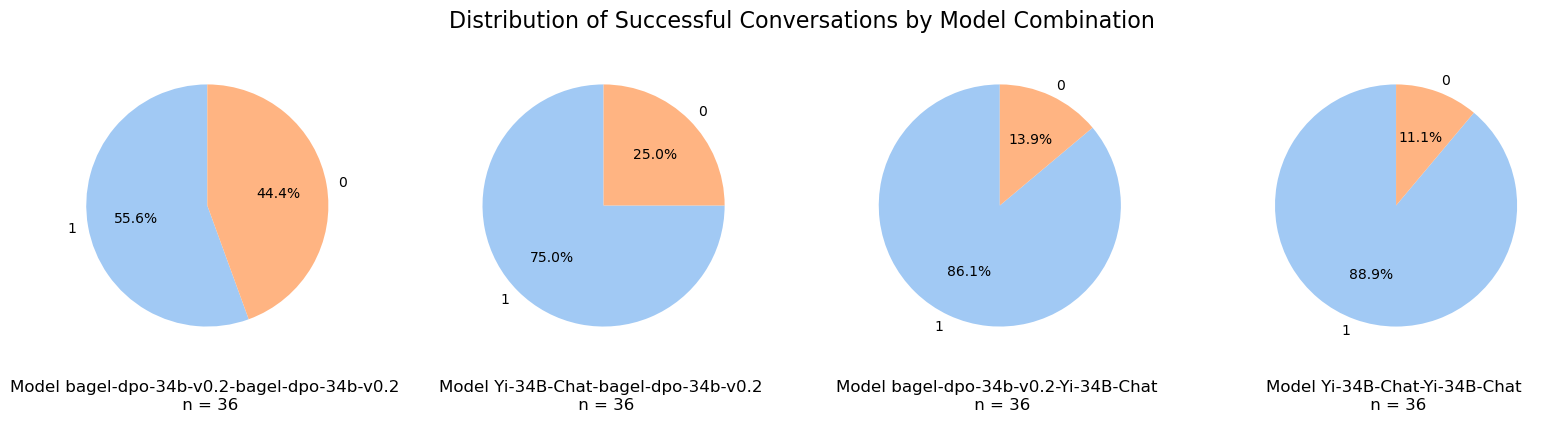
\includegraphics[width=1\textwidth]{plots/pieplot_successful_conversations.png}
    \caption[eval]{Distribution Of Successful Conversations By Model Combination}
    \label{fig:success_conversations}
\end{figure}


\begin{figure}[h]
    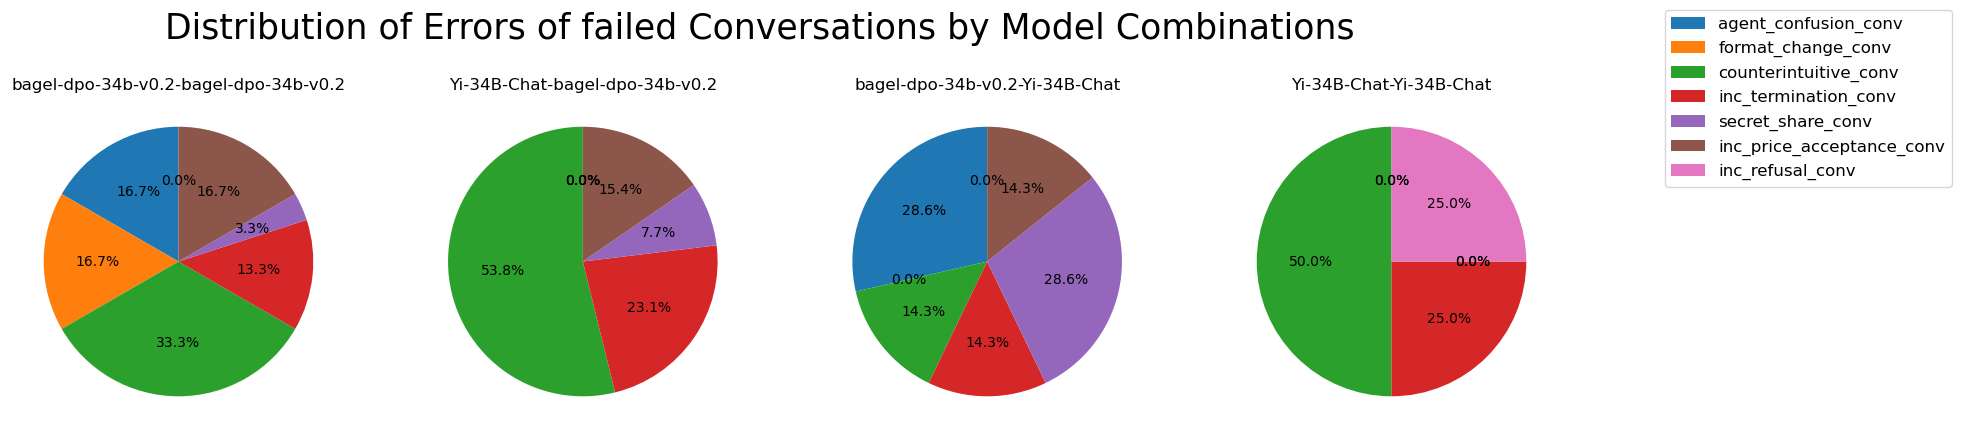
\includegraphics[width=1\textwidth]{plots/pieplot_failed_conversations_errors.png}
    \caption[eval]{Distribution Of Errors Of failed Conversations By Model Combinations}
    \label{fig:failed_conv_errors}
\end{figure}

\begin{figure}[H]
    \centering
    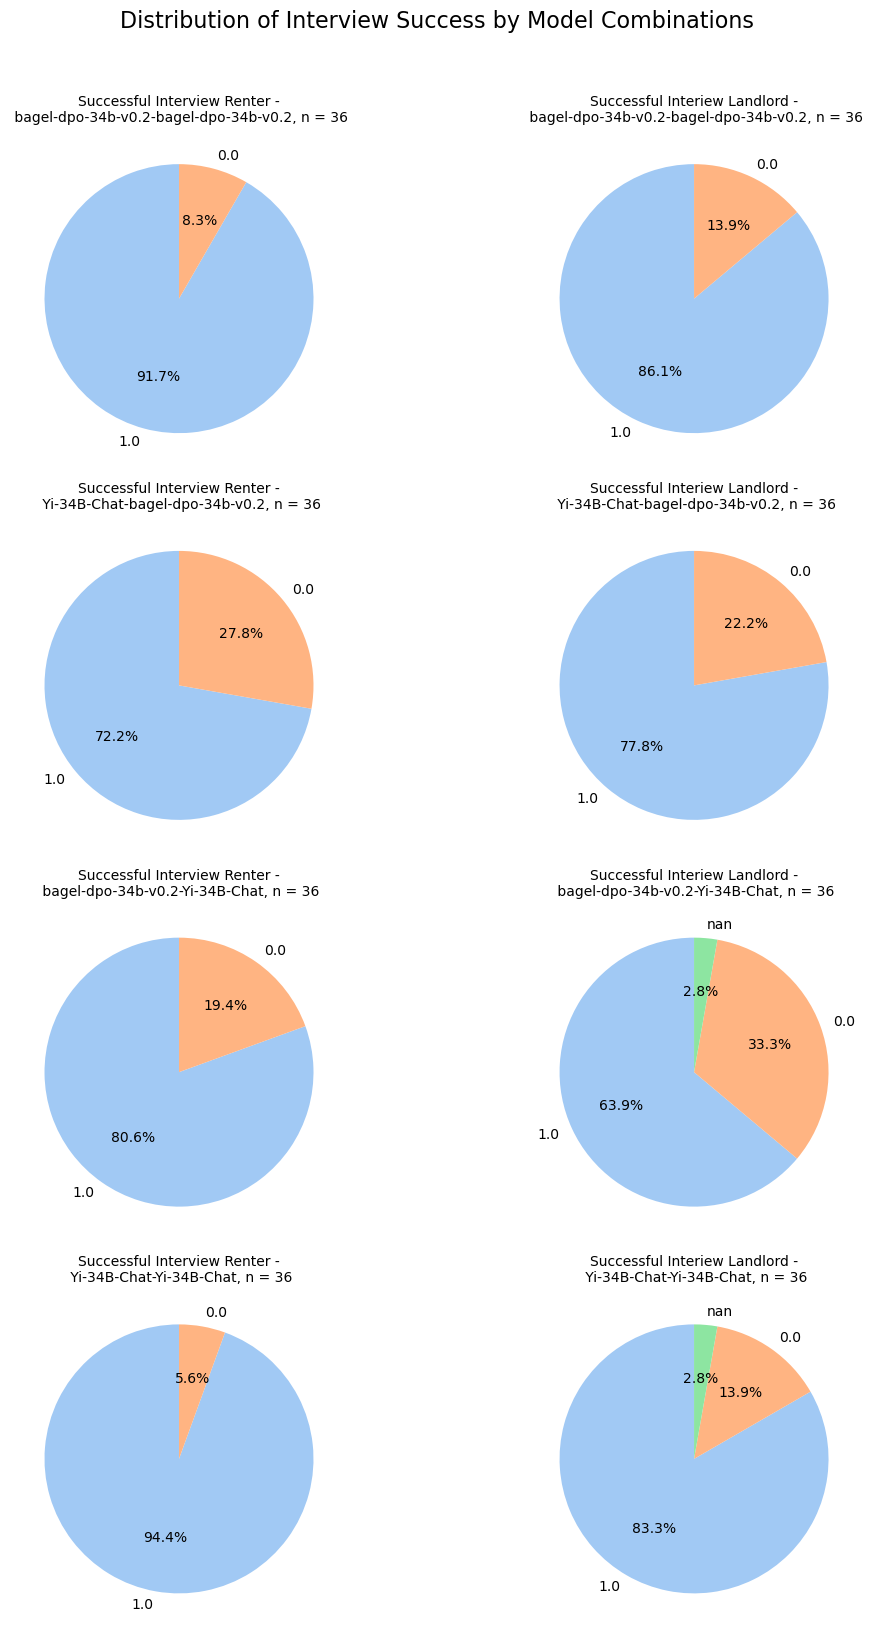
\includegraphics[keepaspectratio=true,scale=0.5]{plots/pieplot_successful_interviews.png}
    \caption[eval]{Distribution Of Interview Success By Model Combinations}
    \label{fig:success_interviews}
\end{figure} 





\newpage

\section{Quantitative Analysis Results}
\begin{figure}[h]
    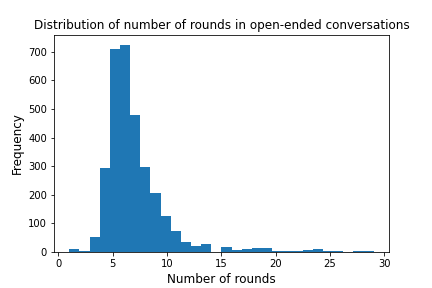
\includegraphics[width=1\textwidth]{plots/histogram_open-ended.png}
    \caption[eval]{Number Of Conversation Rounds In Open-Ended Negotiations}
    \label{fig:histogramm_rounds}
\end{figure}
\begin{figure}[h]
    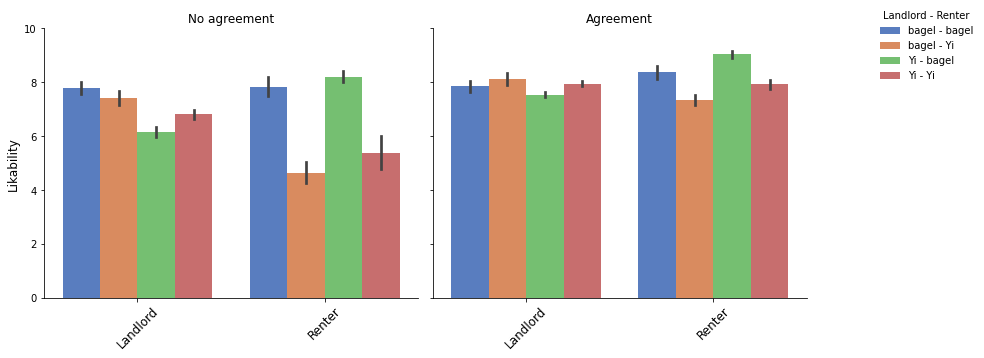
\includegraphics[width=1\textwidth]{plots/agreement_likability_bar.png}
    \caption[eval]{Assigned Likability To Conversation Partner}
    \label{fig:agreement_likability}
\end{figure}

\begin{figure}[h]
    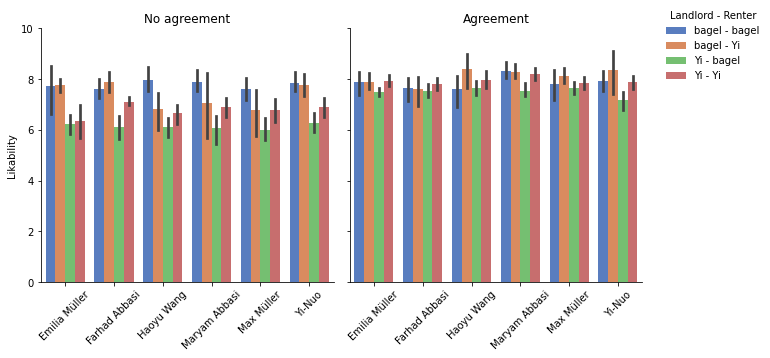
\includegraphics[width=1\textwidth]{plots/landlord_assigned_likes_bar_cross_model.png}
    \caption[eval]{Assigned Likability Scores To Renters By Landlord Peter Schmidt}
    \label{fig:agreement_likability_landlord}
\end{figure}

\begin{figure}[h]
    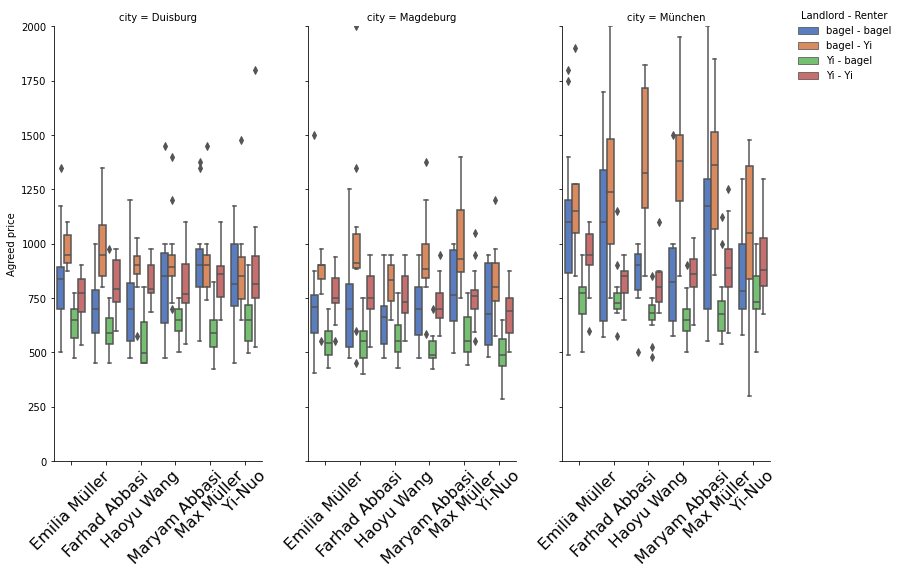
\includegraphics[width=1\textwidth]{plots/agreed_pricesanswer_name.png}
    \caption[eval]{Agreed Prices By Renter Name}
    \label{fig:name_agreedprice}
\end{figure}

\begin{figure}[h]
    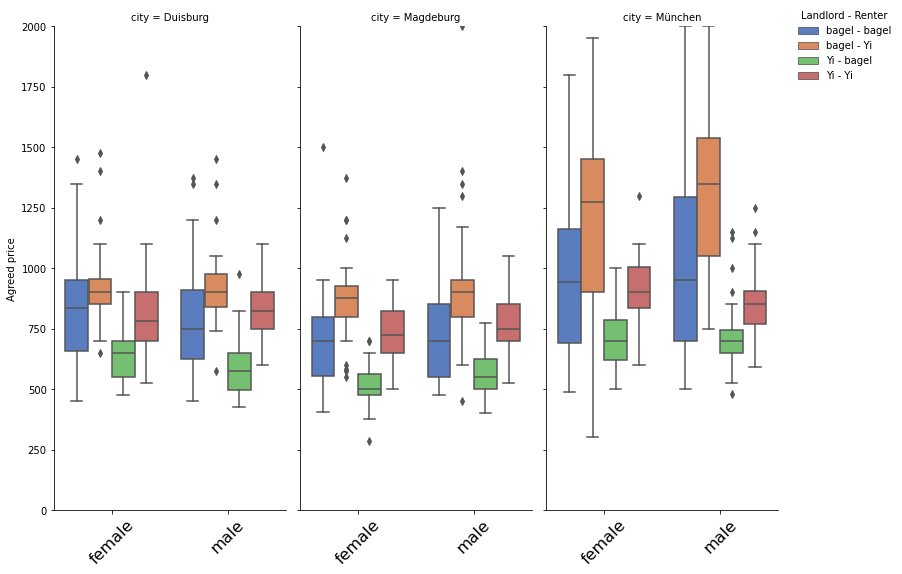
\includegraphics[width=1\textwidth]{plots/agreed_pricesgender.png}
    \caption[eval]{Agreed Prices By Gender Of Renter}
    \label{fig:gender_agreedprice}
\end{figure}

\begin{figure}[h]
    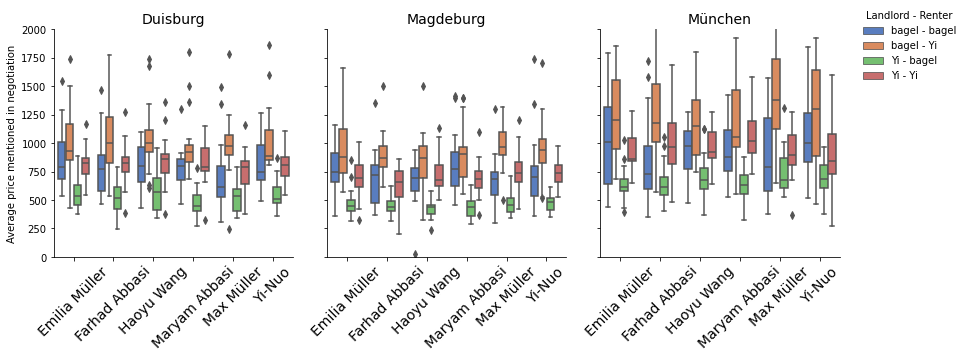
\includegraphics[width=1\textwidth]{plots/name_box.png}
    \caption[eval]{Average Discussed Prices By Name Of Renter}
    \label{fig:name_avgprice}
\end{figure}

\begin{figure}[h]
    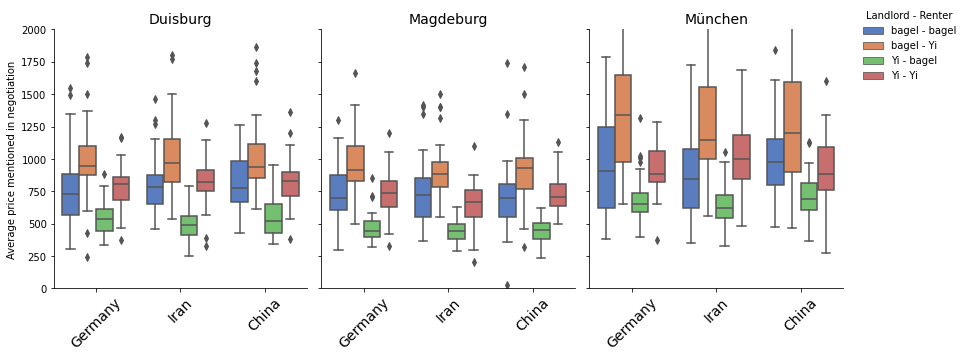
\includegraphics[width=1\textwidth]{plots/country_box.png}
    \caption[eval]{Average Discussed Prices By Country Of Renter}
    \label{fig:country_avgprice}
\end{figure}

\begin{figure}[h]
    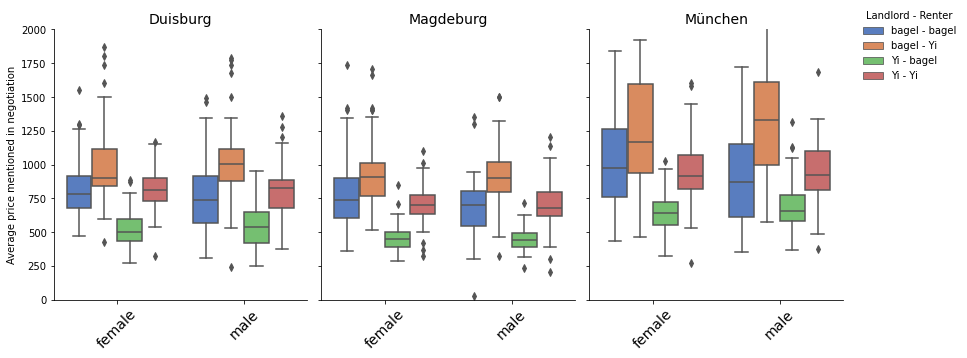
\includegraphics[width=1\textwidth]{plots/gender_box.png}
    \caption[eval]{Average Discussed Prices By Gender Of Renter}
    \label{fig:gender_avgprice}
\end{figure}

\end{document}
